\documentclass[12pt,a4paper]{article}
\usepackage[UTF8]{ctex}
\usepackage{geometry}
\usepackage{graphicx}
\usepackage{float}
\usepackage{amsmath}
\usepackage{amsfonts}
\usepackage{amssymb}
\usepackage{booktabs}
\usepackage{multirow}
\usepackage{array}
\usepackage{longtable}
\usepackage{enumerate}
\usepackage{fancyhdr}
\usepackage{lastpage}
\usepackage{hyperref}
\usepackage[normalem]{ulem}

% 页面设置
\geometry{left=2.5cm,right=2.5cm,top=2.5cm,bottom=2.5cm}
\setlength{\headheight}{15pt}

% 页眉页脚设置
\pagestyle{fancy}
\fancyhf{}
\fancyhead[C]{实\hspace{0.5em}验\hspace{0.5em}原\hspace{0.5em}始\hspace{0.5em}记\hspace{0.5em}录}
\fancyfoot[L]{\parbox[t]{\textwidth}{实验人员：\underline{陈恪瑾}  学号：\underline{U202413925}  同组人员：\underline{黄伟峰}}}
\fancyfoot[R]{教师签字：\underline{\hspace{3cm}}}

\begin{document}

% 正文第一行标题
\noindent
{\Large \textbf{实验九：}\underline{\textbf{一阶电路的响应}}} \hfill {\Large \textbf{实验台编号：}\underline{\textbf{05}}}
\vspace{0.5cm}

\section*{一、实验注意事项}
\begin{enumerate}
    \item 测试用时的信号源要调成正方波，即将方波的offset设为5V。
    
    \item 用取样电阻测电流时，可以通过波形获取方式设置为"平均值"的方法。
    
    \item 可以利用示波器对波形的数字运算功能对电阻R两端电位做减法运算，测电位差来测试RO串联电路的电流波形。
    
    \item 示波器、信号发生器的公共端与电路中的"GND"必须连接在一起。。
\end{enumerate}

\section*{二、实验线路}
\begin{figure}[H]
    \centering
    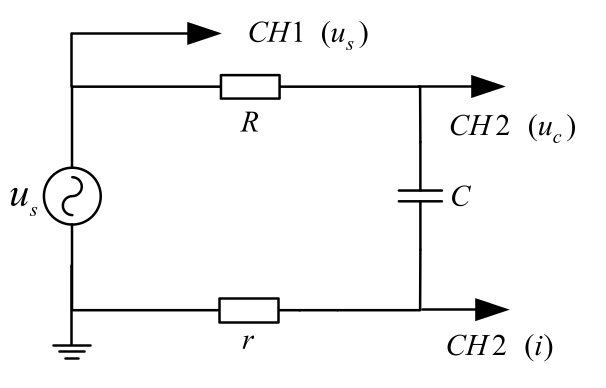
\includegraphics[width=0.8\textwidth]{templete_preview/1.png}
    \caption{实验线路图}
    \label{fig:circuit}
\end{figure}

\section*{三、拍照记录}
\begin{enumerate}

    \item $R = 1k\Omega, 5k\Omega, 10k\Omega$下的电压、电流波形响应。
\end{enumerate}

\end{document}
